\documentclass{beamer}

\usetheme[]{Rochester}
\usecolortheme{beaver}
\usepackage[latin1]{inputenc}
\usepackage{graphics}

\author{Will Webberley}
\date{Autumn 2014}
\institute[COMSC]{Cardiff School of Computer Science and Informatics}



\title{Generating Designs and Prototyping}
\subtitle{CM2101: Human-Computer Interaction}

\begin{document}

\frame{\titlepage}
    
\frame{
    \frametitle{Generating designs}
    \begin{columns}
        \column{.5\textwidth}
            \begin{itemize}
                \item Iterative process important part of interaction design cycle
                \item `Entry point' for iterative cycle
                \item Design is conceptual (brings together ideas)
                \item Requires either:
                \begin{itemize}
                    \item Initial needs / requirements
                    \item Evaluation from previous iteration
                \end{itemize}
                \item ... Before the design can be implemented
            \end{itemize}
        \column{.5\textwidth}
            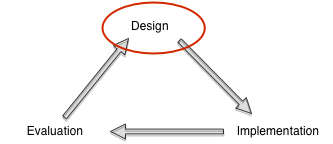
\includegraphics[width=5cm]{media/cycle_3.png}
    \end{columns}
}   

\frame{
    \frametitle{Conceptual design}
    \begin{center}
        A descriptio
    \begin{itemize}
        \item Turn user requirements into a conceptual model
        \item 
    \end{itemize}
}

\frame{
    \frametitle{Prototype implementation}
    \begin{columns}
        \column{.5\textwidth}
            \begin{itemize}
                \item Implementation of design
                \item Fidelity of prototype increases with iterations
                \item Take ideas from design and implement into an interface (whether low-fi or high-fi)
                \item This interface can then be evaluated (heuristic, user, cognitive)
                \item ... Before a new design can be formed!
            \end{itemize}
        \column{.5\textwidth}
            % Update this image to `implementation' highlighted:
            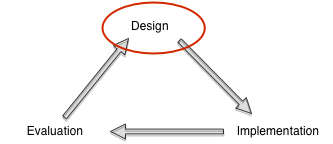
\includegraphics[width=5cm]{media/cycle_3.png}
    \end{columns}
}

\frame{
    \frametitle{Prototypes}
    \textbf{What is a prototype generally?}
    \begin{columns}
        \column{.5\textwidth}
            \begin{itemize}
                \item Initial `versions' during development
                \item Used for evaluation before improvement or release
                \item Often \textit{not} the released version
                \item e.g. a concept car
            \end{itemize}
        \column{.5\textwidth}
            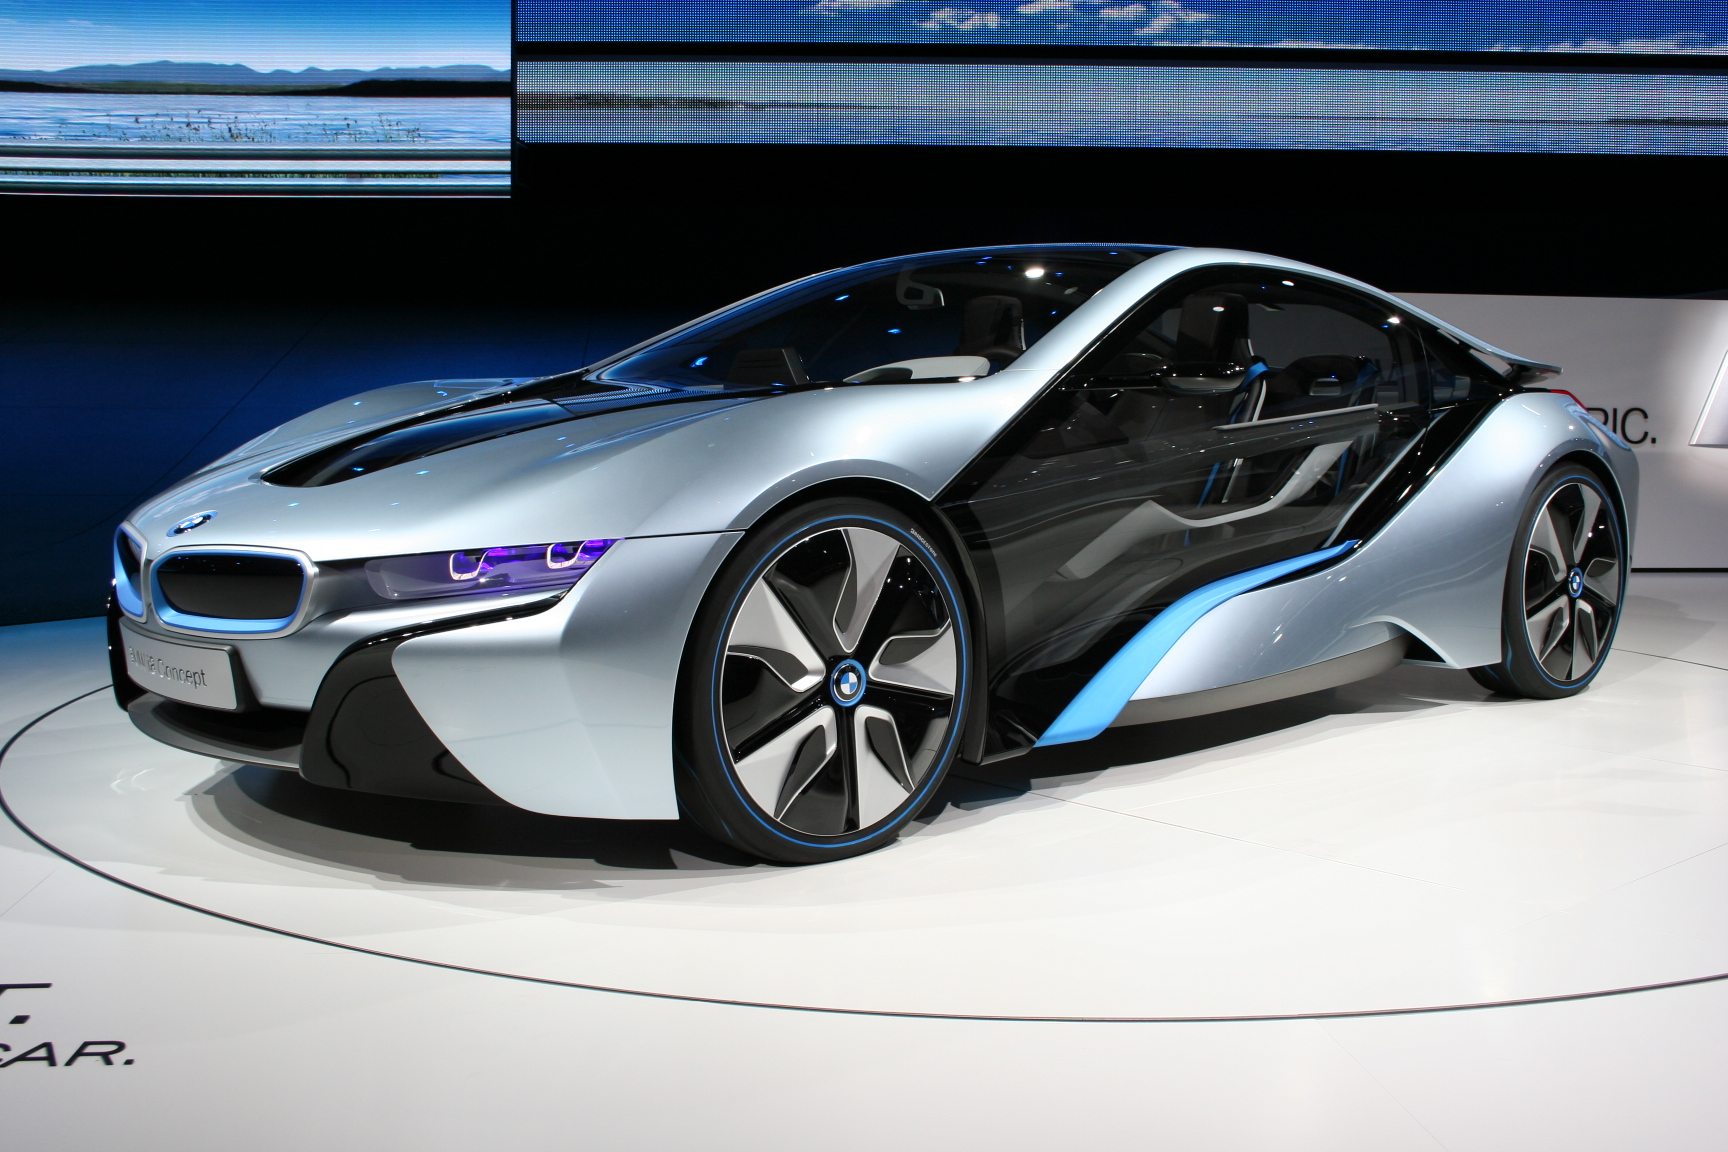
\includegraphics[width=5cm]{media/i8_prototype.jpg}
    \end{columns}
}

\frame{
    \frametitle{Prototypes}
    \textbf{What is a prototype in interaction design?}
    \begin{columns}
        \column{.5\textwidth}
            \begin{itemize}
                \item Early versions of interfaces
                \item Storyboards
                \item Initial sketches of UI
                \item Video simulation
                \item Higher-fidelity mockups
                \item Early versions of implemented software
            \end{itemize}
        \column{.5\textwidth}
            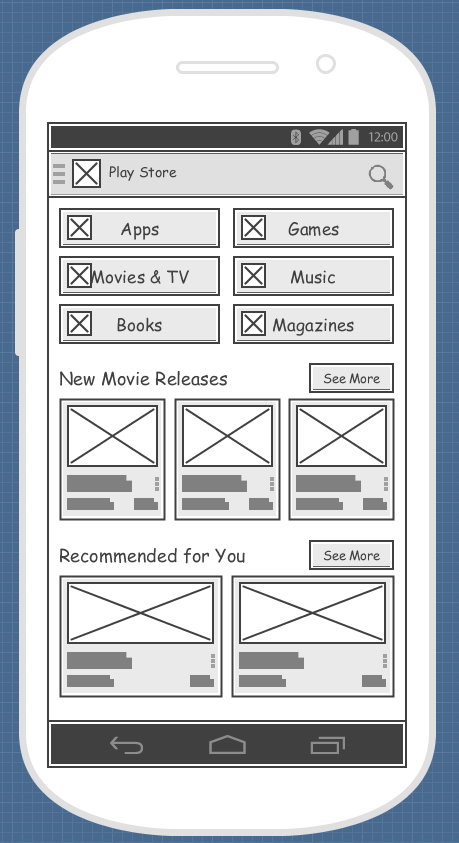
\includegraphics[width=3cm]{media/vp_wireframe.png}
    \end{columns}
}

\frame{
    \frametitle{Why prototype?}
    \begin{itemize}
        \item \alert{Essential} for evaluation and gaining feedback
        \item Allows for testing ideas very quickly
        \item Answer questions and allow for choosing between designs
        \item Stakeholders can interact and understand prototypes more easily than written lists or drawings
        \item Allow team members to communicate ideas clearly
    \end{itemize}
}

\frame{
    \frametitle{What does prototyping capture?}
    \textbf{Prototyping encapsulates}
    \begin{itemize}
        \item Task design
        \begin{itemize}
            \item Methods
            \item Operator ordering (workflow)
            \item Goals and sub-goals
        \end{itemize}
        \item Technical issues (revealed when prototype is later \textit{evaluated}
        \item Usability issues (revealed when evaluated)
        \item Screen layouts
        \item Difficult-to-explain areas
    \end{itemize}
}

\frame{
    \frametitle{Prototyping: Low-fidelity}
    \begin{columns}
        \column{.7\textwidth}
            \begin{itemize}
                \item First-mid cycles in iterative design
                \item Very cheap
                \item Very quick to develop and turn around (easily changed)
                \item Use a medium unlike final product (e.g. whiteboard, paper, post-its, digital sketches)
                \item Design team meet together and bash out ideas
                \item Limited functionality but...
                \begin{itemize}
                    \item Highlights ordering of tasks
                    \item Identifies where requirements met
                \end{itemize}
            \end{itemize}
        \column{.3\textwidth}
            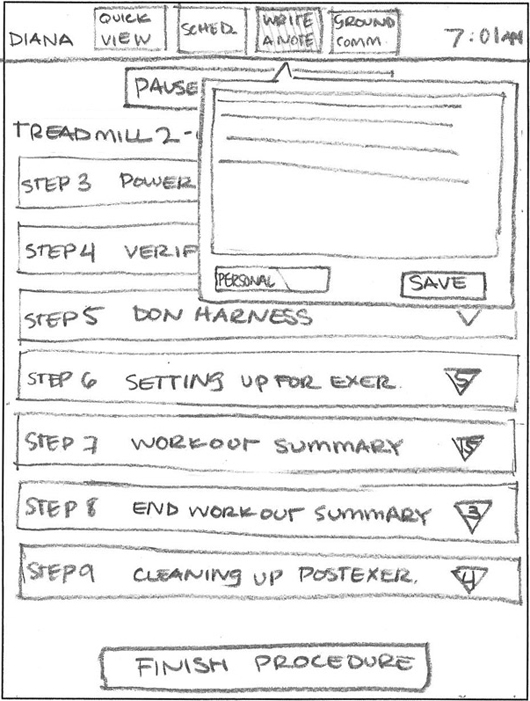
\includegraphics[width=3cm]{media/lowfi_prototype.jpg}
    \end{columns}
}

\frame{
    \frametitle{Prototyping: Medium-fidelity}
    \begin{columns}
        \column{.7\textwidth}
            \begin{itemize}
                \item Mid-end cycles in iterative design
                \item More expensive and slower than low-fi
                \item But still allows for quicker implementation-evaluation cycle than high-fi
                \item 100\% digital (usually in a GUI builder or wireframing tool)
                \item Use UI components and controls specific to the platform
                \item Follow platform guidelines
                \item Can still incorporate new requirements
            \end{itemize}
        \column{.3\textwidth}
            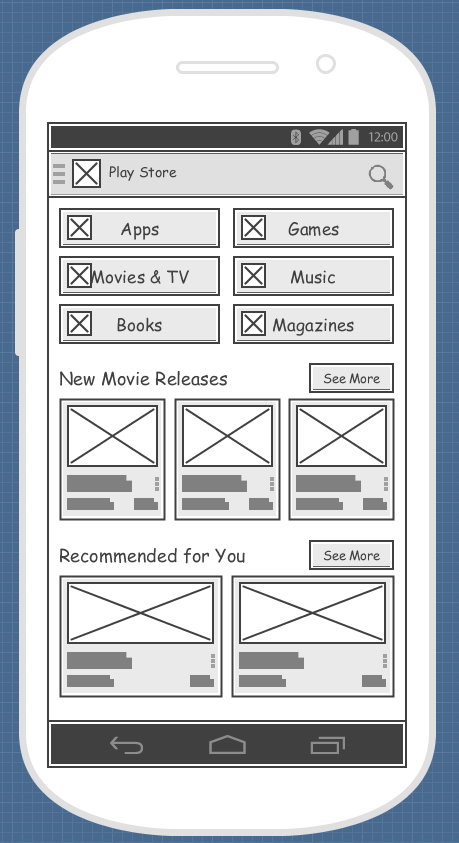
\includegraphics[width=3cm]{media/vp_wireframe.png}
    \end{columns}
}

\frame{
    \frametitle{Prototyping: High-fidelity}
    \begin{columns}
        \column{.5\textwidth}
            \begin{itemize}
                \item Final cycles in iterative design
                \item Usually as buggy implementations (or towards final product)
                \item Slower cycles
                \item More expensive (as a `working' product produced in each cycle)
                \item Inappropriate to incorporate new requirements (scope creep)
            \end{itemize}
        \column{.5\textwidth}
            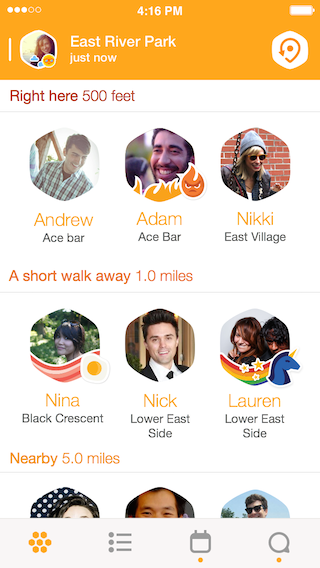
\includegraphics[width=4cm]{media/swarm.png}
    \end{columns}
}

\frame{
    \frametitle{Prototype compromise}
    \textbf{Every prototype is inherently compromised}
    \begin{itemize}
        \item System dependent features not considered
        \begin{itemize}
            \item Response time
            \item Hardware functionality
            \item This is why evaluation is important afterwards
        \end{itemize}
        \item \alert{Horizontal} compromise (think: shallow HTA)
        \begin{itemize}
            \item Implement design for wide range of functions
            \item Each function is prototyped with limited detail
        \end{itemize}
        \item \alert{Vertical} compromise (think: deep HTA)
        \begin{itemize}
            \item Implement design for small number of functions
            \item Each function is prototyped with great detail
        \end{itemize}
        \item Compromises should be \alert{ignored}: products need to be \textit{engineered}
    \end{itemize}
}

\frame{
     \frametitle{Revision questions}
     \begin{enumerate}
        \item
     \end{enumerate}
}

\frame{
    \frametitle{Summary}
    \begin{itemize}
        \item
    \end{itemize}
}    

\end{document}
